\begin{table}[t]
\centering
\scriptsize
\resizebox{\columnwidth}{!}{
\begin{tabular}{|l|l|} \hline
\textbf{Application}& \textbf{Description}\\
\hline
Prophet& Time series decomposition and prediction\\ 
\hline
Multi-Regression& Multiple linear regression/prediction of time series\\
\hline
XGBoost& Regression and classification by gradient boosting\\
\hline
SVC & Classification based on support vector machine\\
\hline
Neural Network& Classification by layered artificial neural network\\
\hline
\end{tabular}}
\caption{Machine learning applications used as benchmarks
to evaluate Seneca. 
%paper submission is blind (so such references must be omitted so as not to reveal our identities):
%Code base is available at project repository~\cite{ref:seneca}.
\label{tab:bmarks}}
\vspace{-0.2in}
\end{table}

In this section,
we evaluate Seneca in terms of performance, monetary cost, and hyperparameter tuning time (latency), 
using machine learning applications that we ported to Seneca (i.e. that we implemented
as lambda functions). 
We first overview these applications and our empirical methodology. 
We then present our experimental results. 

\subsection{Benchmark Applications and Training/Testing  Datasets}
The machine learning applications that we use to evaluate Seneca 
are shown in Table~\ref{tab:bmarks}, each with 
a brief description.
Prophet~\cite{ref:prophet} is a time series analysis library built and maintained by Facebook and the open-source community. The input dataset is a time series of view counts
%logorithm
of Payton Manning's wikipedia page from Dec. 10th, 2007 to Jan. 20th, 2016. 
The dataset exhibits both seasonality and a holiday effect (e.g. around the super bowl games). 
We use the first 6 years as the training set and the last 2 years as the testing set.
We use a cross-validation horizon (sliding window) of 1-year, 
and a period (sliding pace) 
of 180 days.  As such, Seneca performs three cross-validations for each 2-year testing range.

%%The hyperparameters that Prophet expects are 
%%\textcolor{blue}{Describe what these are in a couple of sentences.}
%%In the results that follow, we evaluate \textit{default} parameteterizations (that come with 
%%the application or that are defined by the application developer) for each application.  
%%The default parameters for this application are
%%\textcolor{blue}{Describe them here.}
%%The application computes mean square error of
%%\textcolor{blue}{finish this here.}

Prophet expects multiple hyperparameters: \textit{growth} specifies linear or logistic trend model growth; \textit{prior scale} indicates the strength of the 
sparse prior probability~\cite{ref:sparse_prior}. 
There are three prior scale hyperparameters for change point, holidays, and seasonality. 
Since Prophet uses a Fourier sum to estimate seasonality, 
the \textit{fourier order} is the number of terms in the partial Fourier 
sum. \textit{Seasonality mode} indicates that the effect of seasonality is either 
multiplicative or additive. Finally, the width of uncertainty intervals 
can be set using the hyperparameter \textit{interval width}.

% \textcolor{blue}{Describe what these are in a couple of sentences.}
In the results that follow, we evaluate \textit{default} parameteterizations (that come with 
the application or that are defined by the application developer) for each application.  
The default parameters and tuning options for this application are listed in the table~\ref{tab:prophet_para}. For every cross validation, the application computes mean square error (MSE) as $\frac{1}{n}\sum_{i=1}^{n}(Y_i - \hat{Y_i})$, where $\hat{Y_i}$ is the ground truth, $Y_i$ is model prediction and n is the number of data points. Then the application returns the average MSE of all cross validation. Based on the model trained by default parameter setting, this average MSE metric is 0.284.

\begin{table}[t]
\centering
\scriptsize
\resizebox{\columnwidth}{!}{
\begin{tabular}{|l|l|l|} 
\hline
\textbf{Hyperparameter}& \textbf{Default} & \textbf{Tuning options}\\
\hline
grow & linear & [linear, logistic] \\
\hline
changepoint prior scale & 0.05 & [0.05, 0.5] \\
\hline
holidays prior scale & 10 & [1, 5, 10] \\
\hline
seasonality prior scale & 0.5 & [0.1, 0.5] \\
\hline
fourier order & 10 & [5, 10, 15, 20] \\
\hline
seasonality mode & additive & [additive, multiplicative] \\
\hline
interval width & 0.8 & [0.5, 0.8] \\
\hline
\end{tabular}}
\caption{The selected configurable hyperparameters of Prophet. The default value and tuning options are listed. 
\label{tab:prophet_para}}
\vspace{-0.2in}
\end{table}


Multi-Regression is a regression application 
from an IoT project~\cite{iot-cpu} that was developed by the authors
to predict outdoor temperature from the processor 
temperature of single board computers (SBCs).  
The technique uses multiple linear regression models computed from time
series of processor temperature measurements,
to predict outdoor microclimate temperatures (e.g. for use in 
precision agriculture applications such as irrigation control and frost protection).
The training dataset consists of eight input time series (one per SBC, each containing 
5-minute measurements) from April 5th, 2018 to Dec. 10th, 2018.

A hyperparameter configuration for this application is a subset of input SBC time series.
Seneca considers all \texttt{$2^N - 1$} potential subsets (for $N$ input time series).
For this application,
we assume the default parameterization is the set of all $N$ input time series (8 in this case).
The test dataset for this application is a time series of the outdoor temperature (ground truth) 
over the same period.  The application makes predictions for each of these outdoor temperatures
using the model constructed from the training set
and computes the mean square error across predicted and ground truth value pairs.

XGBoost~\cite{ref:xgboost-web} is an open source framework for gradient boosting, which 
performs both regression and classification. We consider it a regression application and
a classification application in this evaluation.  
Support vector classification (SVC)~\cite{ref:svc} is a classification algorithm 
based on support vector machine and implemented by libsvm~\cite{ref:libsvm} library.
Neural network~\cite{ref:neural_network} is a machine learning framework that learns 
and make decisions from patterns in an input dataset. For this application, 
we use a feedforward multilayer perceptron model~\cite{ref:feedforward_nn} 
for the classification task.

For these applications (XGBoost, SVC, and Neural Network), 
we use a labeled dataset for training, testing, and evaluation from 
this project~\cite{iot-cpu}. The dataset contains
measurements from individual citrus fruit (e.g. oranges, mandarins, lemons, etc.) 
taken by a fruit sorting and grading device (using a large number of sensors).  
The measurements (i.e. features)
include size, shape, weight, color, diameter, flatness, among other characteristics,
for each fruit.  The label indicates which field the fruit was harvested from.  
The applications train a model on a random subset of the data.  
They then use this model to predict the field
%%<<<<<<< HEAD
%%from which each fruit originates.  They compute classification accuracy 
%%as \textcolor{blue}{finish this.}.  XGBoost also computes MSE for its regression task
%%on the same datasets.  The dataset has been filtered authors to remove correlated 
%%features (those with an absolute value of the Pearson correlation coefficient greater than 0.8).  
%%The resulting dataset contains 218150 rows (individual fruit) each with 19 features. 
from which each fruit originates. They compute classification accuracy score as $\frac{1}{n}\sum_{i=1}^{n}1(Y_i = \hat{Y_i})$, where $Y_i$ is the prediction class, $Y_i$ is the true class, n is the number of samples and 1(x) is the indicator function. XGBoost also computes MSE for its regression task on the same datasets. The dataset has been filtered to remove correlated features (those with an absolute value of the Pearson correlation coefficient greater than 0.8). The dataset has also been balanced by downsampling one target whose number greatly exceeds other ones. The resulting dataset contains 33926 rows (individual fruit) distributed evenly to 5 targets and each row has 18 features.

%The dataset is from a Compac packline machine~\cite{ref:compac} that sorts and grades fruit using a large number of 
%measurements (i.e. feature measurements including size, shape, weight, color, diameter, flatness, etc.).  The labels identify the field from which fruit was harvested.
%The dataset is filtered to remove correlated features (those with an absolute value of the Pearson correlation 
%coefficient greater than 0.8).  

%Seneca downloads the dataset from AWS S3 for each function invocation.
%It then randomly indexes the data set and splits it into two.  
For these applications (XGBoost, SVC, and Neural Network), we consider three split scenarios for training and testing: 80\%-20\%, 20\%-80\% and 0.1\%-99.9\%. As the proportion of training data decreases, the performance of classifier degrades accordingly and we argue that Seneca is able to eke out improvement even with very limited training data.
%\textcolor{blue}{list them here once we finish the additional results} 
%This setup also means that each Seneca function
%considers a different training and testing set during hyperparameter tuning. 

%todo in the future -- for a complete tuning, use the same testing and training sets
%run this multiple times (for the same test/train datasets) and report the average and stdev in the latency (and memory?) results.
%todo in the future -- repeat the above using different test/train datasets, but keep 
%them the same for all functions in a single tuning run.  Compare the MSE/accuracy and
%the configurations that are selected, analyze how they change (if they do)

\subsection{Empirical Methodology}
To evaluate Seneca, we measure tuning performance, application execution time, and monetary cost.
For tuning performance, we use mean squared error (MSE) for regression tasks 
and percentage accuracy for
classification tasks. The default configuration that we 
consider for each application is described above.
We report results for the default, best (Seneca's recommendation), 
and worst performing configurations.  Seneca computes all possible combinations 
of the hyperparameter settings specified in the configuration to extract each of these results.
The default results represents those that a novice or first time 
user might employ when using these applications
as a "black box".  The worst performing scenario shows how bad the results can be
when parameters are poorly tuned.  Finally, the best is the upper bound on what is possible from 
tuning the hyperparameters (e.g. using expert knowledge or Seneca). 

We deploy Seneca on Amazon Web Services (AWS) Lambda and extract
execution time and memory use from AWS CloudWatch logs.  We then compute monetary cost
using the AWS Lambda pricing model~\cite{ref:pricing}.
%awslambdapricing: https://aws.amazon.com/lambda/pricing/
Each function downloads the training and testing dataset 
of the application from AWS Simple Storage Service (S3) upon function invocation. 
We do not consider the cost of dataset storage in our cost computations (it is very small).

We also experiment with different memory configurations for Seneca functions in AWS Lambda.  
We evaluate
the performance and cost of allocating the maximum memory for each and for automatically optimizing 
memory use using Seneca. We assume that all combinations hyperparameter settings use the 
same maximum amount of memory across functions; we 
have verified that this assumption holds for the applications and datasets we consider.
We plan to consider applications for which hyperparameter settings require 
different maximum amounts of memory as part of future work.  

\subsection{Tuning Performance}

\begin{table}
\centering
\begin{tabular}{|c|c|c|c|}
\hline
& Prophet & Multi-Regression & XGBoost\\
\hline
\# of Combinations & 384 & 255 & 768\\
\hline
\hline
Default MSE & 0.284 & 11.446 & 0.119 \\
\hline
Worst MSE & 1.266 & 43.752 & 8.98 \\
\hline
Best MSE (Seneca) & 0.220 & 9.621 & 0.044 \\
\hline
%percent difference between default and best 26.07%, 15.94%, 67.30%
%percent difference between worst and best 82.63%, 78.01%, 95.52%
%\begin{figure}[t] \centering 
%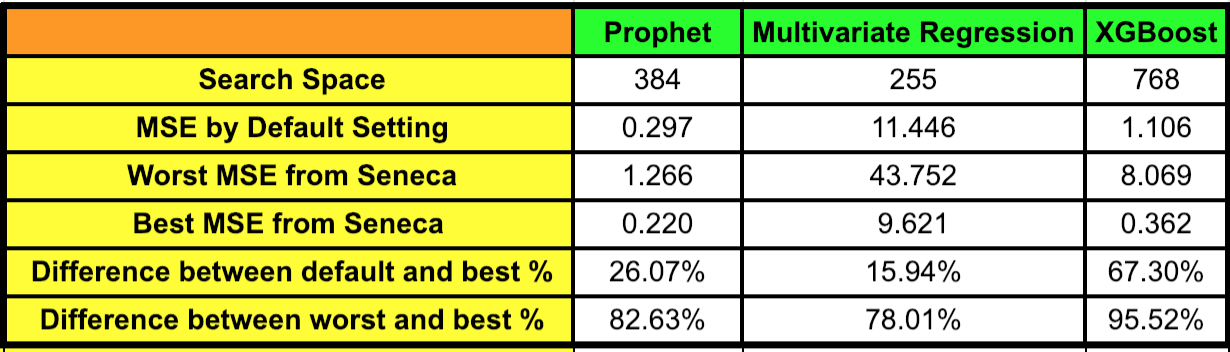
\includegraphics[scale=0.4]{mse}
\end{tabular}
\caption{Combination count and MSE for the default, best (Seneca's recommendation), and worst hyperparameter configurations for the three regression applications. 
For the MSE  values (rows 3-5), lower is better.
\label{tab:mse}}
\end{table}

\begin{figure}[t] \centering 
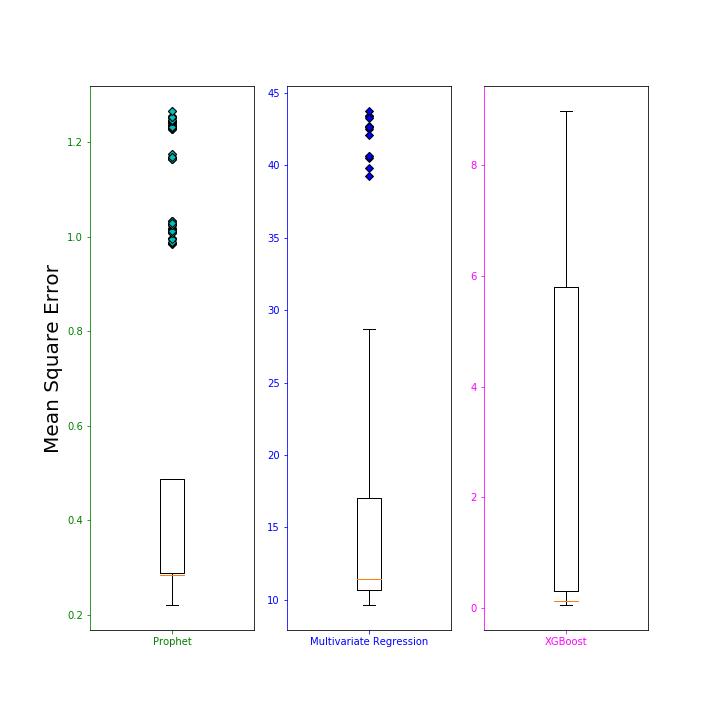
\includegraphics[scale=0.36]{box_plot_mse_2}
\caption{The box plot of MSE metric from three regression applications in the entire hyperparameter tuning search space. The red notch shows the MSE from the default settings. The colored diamonds are outliers beyond two interquartile ranges. Lower MSE values are better.
\label{fig:box_plot_mse}}
\vspace{-0.2in}
\end{figure}

We first evaluate Seneca using the three regression applications: 
Prophet, Multi-Regression, and XGBoost (regression task). 
Table ~\ref{tab:mse} shows the size of the hyperparameter search space (number of configurations
considered) and the mean squared error (MSE)
for each of the regression applications that we consider (columns 3-5).
The first row of data is 
 the number of hyperparameter configurations in the search space of each. 
The last three rows show the MSE for the default, worst, and best performing 
hyperparameter configuation reported by Seneca (lower is better).  
Note that Seneca's recommendation is the best performing configuration.
Seneca reduces MSE by 26\%, 16\%, and 63\%, for Prophet, Multi-Regression, and XGBoost,
respectively, for the datasets and training methodologies that we consider.
Verses the worst case, Seneca reduces MSE by 83\%, 78\%, and 99\%, respectively.


Figure~\ref{fig:box_plot_mse} provides a box plot of MSE (lower is better)
for these applications 
for the entire hyperparameter 
search space. The central rectangle covers the interquartile range (IQR), 
which is defined as the range of data 
points from first quartile to third quartile (Q3 - Q1). 
The upper whisker extends to the last datum less 
than \texttt{$(Q3 + 2 * IQR)$} and the lower whisker extends to the first datum greater 
than \texttt{$(Q1 - 2 * IQR)$}. The data points beyond the whiskers are considered outliers 
and are plotted as colored diamonds. The red notch identifies the MSE that results from training 
the model using the default settings of hyperparameter. The difference between red notch of lowest data 
point is improvement brought about through the use of Seneca. From the location of red notch, we can see the MSE metrics from default configuration in three applications are close to the first quartile value, meaning the potential room for improvement is about 75\% over the range of MSE metric. The box plot also illustrates that the best MSE of Prophet and multivariate regression are among outliers, where a comprehensive search is very critical to find the best configurations. 
%\textcolor{blue}{Add more analysis here to discuss the variance in the MSE for the range of configurations and how they change across applications. Include any insights that the boxplots add.}

%%%%%%%%%%%%%%%%%%%%% classification apps - tuning performance %%%%%%%%%%%%%%%%%%%%%%%%%
We next empirically evaluate the tuning performance of Seneca for the three
classification applications: XGBoost (classification), SVC, and Neural Network.
Table~\ref{tab:accuracy} presents the accuracy percentage (higher is better) 
reported by each application (3 right-most columns) 
for the default, worst, and best hyperparameter tuning configurations under three training and testing split scenarios reported by Seneca.  
In the 80/20 percent split case, Seneca increases accuracy by 3.43\%, 62.52\%, and 0.53\%, for XGBoost (classification), 
SVC, and Neural Network applications,
respectively.
Verses the worst case, Seneca improves accuracy by 99.13\%, 75.75\%, and 65.57\%, respectively.


\begin{table}
\centering
\begin{tabular}{|c|c|c|c|}
\hline
\textbf{80\%-20\%} & XGBoost & SVC & Neural Network\\
\hline
\hline
Default Accuracy & 95.70\% & 21.77\% & 84.23\%\\
\hline
Worst Accuracy&0.00\%&7.53\% & 19.19\%\\
\hline
Best Accuracy (Seneca) &99.13\% & 83.29\% & 84.76\%\\
\hline
\hline
\textbf{20\%-80\%} & XGBoost & SVC & Neural Network\\
\hline
Default Accuracy & 95.07\% & 21.31\% & 55.44\%\\
\hline
Worst Accuracy&0.00\% & 9.42\% & 19.55\%\\
\hline
Best Accuracy (Seneca) & 98.68\% & 43.61\% & 60.89\%\\
\hline
\hline
\textbf{0.1\%-99.9\%} & XGBoost & SVC & Neural Network\\
\hline
Default Accuracy & 86.37\% & 20.02\% & 20.00\%\\
\hline
Worst Accuracy & 0.00\% & 19.99\% & 19.79\%\\
\hline
Best Accuracy (Seneca) & 89.14\% & 55.79\% & 29.99\%\\
\hline

%percent difference between default and best 83.65%, 83.84%, 79.83%
%percent difference between worst and best 86.07%, 85.73%, 84.63%
%\begin{figure}[t] \centering 
%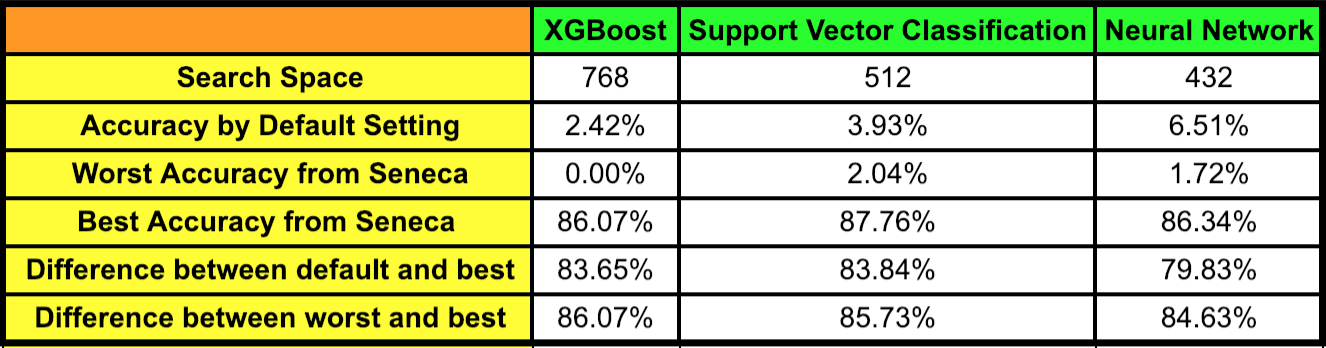
\includegraphics[scale=0.38]{accuracy}
\end{tabular}
\caption{The Accuracy reported for the 
default, best (Seneca's recommendation), and worst hyperparameter configurations for 
the three classification applications under three train/test split scenarios.  
For the accuracy values in the table, higher is better.
\label{tab:accuracy}}
%\vspace{-0.2in}
%\end{figure}
\end{table}

\begin{figure}[t] \centering 
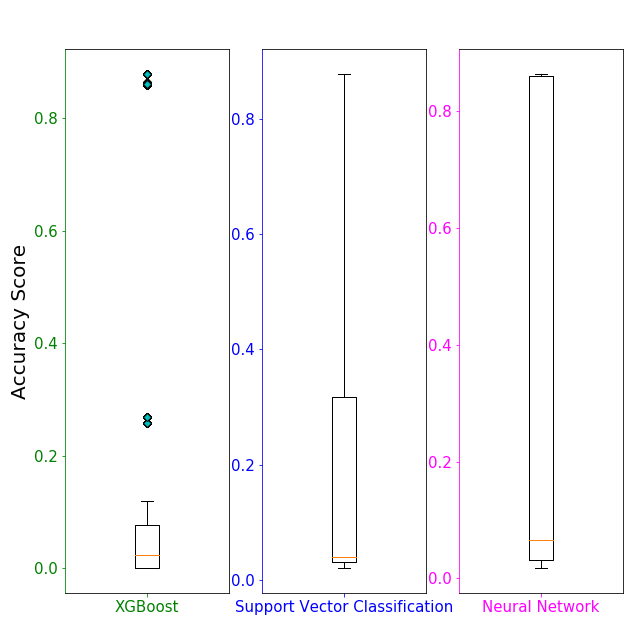
\includegraphics[scale=0.36]{box_plot_accuracy}
\caption{The box plot of accuracy metric from three classification applications for the entire hyperparameter tuning search space. The red notch indicates the accuracy metric from the trained model using default settings. The colorful diamonds are outliers beyond two interquartile ranges. Higher accuracy values are better.
\label{fig:box_plot_accuracy}}
% \vspace{-0.2in}
\end{figure}

Figure~\ref{fig:box_plot_accuracy} presents the accuracy (higher is better) 
for the entire hyperparameter search space for each classification
application.  The central rectangle covers from first quartile to third quartile (Q3 - Q1) and the whiskers span from \texttt{$(Q3 + 2 * IQR)$} to \texttt{$(Q1 - 2 * IQR)$}. The red notch indicates the accuracy metric from the model trained by default settings and colored diamonds are outliers beyond whiskers.
For both types of applications (regression and classification), Seneca significantly
improves tuning performance over the default and worst case configurations for the 
datasets and training methodologies we consider.  

\subsection{Cost Analysis}

We next analyze the monetary cost introduced by Seneca. 
We consider two scenarios for its implementation.
First, we configure each lambda function to use the maximum amount
of memory allowed by AWS Lambda (3008 MB).  Second, we employ Seneca's memory optimization 
which automatically detects and configures the amount of memory needed by each function.
Because memory impacts both cost and execution time (total latency of Seneca hyperparameter tuning), 
we present empirically evaluate both 
in this subsection.  For each, we only include XGBoost once since its 
performance profile is the same
regardless of whether we are using regression or classification.

\begin{table}
\centering
\begin{tabular}{|c|c|c|c|c|c|}
\hline
& Prophet & MR & XGBoost & SVC & NN\\
\hline
\hline
Exec time (minutes)& 24.96 & 4.18 & 17.48 & 0.91 & 2.49 \\
\hline
Cost of Tuning (\$) & 0.722 & 0.121 & 0.5 & 0.023 & 0.072 \\
\hline
\end{tabular}
\caption{ Monetary cost of using Seneca for hyperparameter tuning when configured to use the maximum amount of memory (3008 MB) possible for each function invocation. 
\label{tab:cost_max_memory}}
\vspace{-0.2in}
\end{table}

\begin{table}
\centering
\begin{tabular}{|c|c|c|c|c|c|}
\hline
& Prophet & MR & XGBoost & SVC & NN\\
\hline
\hline
Exec time (minutes)& 38.7 & 8.72 & 29.07 & 0.91 & 3.17 \\
\hline
Cost of Tuning (\$) &0.62 & 0.086 & 0.354 & 0.007 & 0.056 \\
\hline
Cost of optimization (\$) &0.033 & 0.014 & 0.003 & 0.010 & 0.008 \\
\hline
Total Cost (\$) &0.653 & 0.1 & 0.357 & 0.016 & 0.064 \\
\hline
\end{tabular}
\caption{ Seneca  Memory  Optimization:  The  monetary  cost  of using Seneca for hyperparameter tuning when the amount of memory  used  for  each  function  invocation  is  automatically inferred and set by Seneca.
\label{tab:cost_optimized}}
\vspace{-0.2in}
\end{table}

Tables~\ref{tab:cost_max_memory} and~\ref{tab:cost_optimized} show the results with and without 
the Seneca memory optimization, respectively. In both tables, the five columns identify the 
benchmark applications and the first row is the total execution time in minutes for 
Seneca's hyperparameter tuning for the corresponding application.  
In table~\ref{tab:cost_max_memory}, the second row is total cost of tuning when Seneca's 
lambda functions are configured to use the maximum amount of memory (3008 MB), whereas table~\ref{tab:cost_optimized} demonstrates the additional cost of optimization in the third row 
and total cost on fourth row.
% \textcolor{blue}{See my notes to fix the tables in the caption of these figures.}



% \textcolor{blue}{It would be good here in the Seneca case to also run the applications in the minumum amount of memory discovered by Seneca (ie if we were to run Seneca ahead of time, taking the max memory used by any of the functions per application) -- to show what Seneca is missing.  this assumes you are doing the memory optimization WHILE you are doing the tuning -- if you are not, you can leave this out, but we need to remind the reader at this point how the memory optimization is done by Seneca (we should do this in this paragraph, either way).}

% \textcolor{blue}{Comments: The minimum amount of memory is the "max memory used" value. I tried that out and the execution time increases dramatically at the minimum memory case. I will explore the idea of simultaneous optimization and tuning later}


% \textcolor{red}{state what the columns and rows are; then write up some analysis on what the table data is showing and why. provide analysis for both tables and summarize the key differences between them.}


%The results of maximum memory scenario are shown in Figure~\ref{fig:cost_max_memory}. The max memory used and billed duration are reported by AWS CloudWatch and averaged throughout whole search space for each application. Figure ~\ref{fig:cost_optimized} demonstrates the results of optimized memory scenario. The total cost stems from function optimization and hyperparameter tuning. As a comparison of two scenarios, Figure~\ref{fig:cost_analysis} illustrates the total cost of optimized memory scenario is lower than maximum memory scenario in each application respectively.


\begin{figure}[t] \centering 
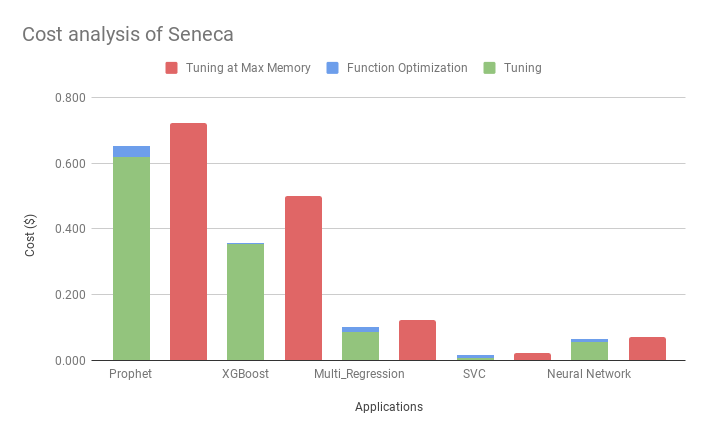
\includegraphics[scale=0.36]{Cost_analysis_2}
\caption{ The cost analysis of Seneca with (Opt) and without (No Opt) the use of its memory optimization. 
By reducing the memory use of each, Seneca reduces the monetary cost of hyperparameter tuning by \textcolor{blue}{X\% on average, across these applications.  *compute and Fill this X in*.}
\textcolor{blue}{Change the legend as follows: change "Tuning at Max Memory" to "No Opt"; change "Function Optimization" to "Opt cost"; change "Tuning" to "Opt". If you can put legend in this order: Opt, Opt cost, No Opt} 
\label{fig:cost_analysis}}
\vspace{-0.2in}
\end{figure}

\begin{figure}[t] \centering 
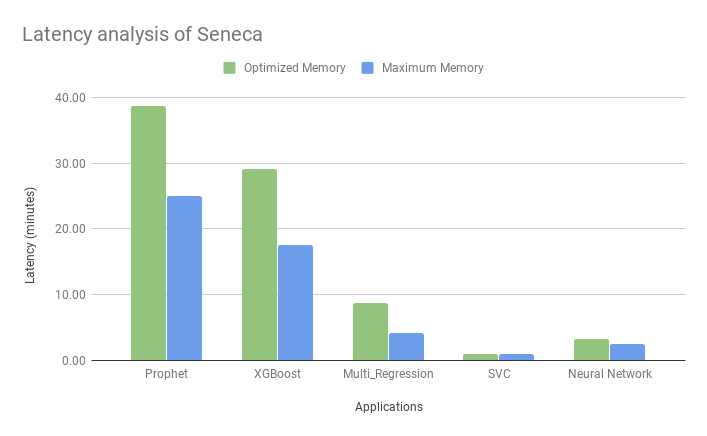
\includegraphics[scale=0.36]{Latency_analysis_2}
\caption{Latency of Seneca with (Opt) and without (No Opt) memory optimization, for each application. As Seneca reduces memory use (and cost), it also extends the execution time of the functions (and thus total tuning time, i.e., the latency of Seneca) by Y\% on average across applications \textcolor{blue}{compute and fill in Y here.}
\textcolor{blue}{Change the legend as follows: change "Optimized Memory" to "Opt"; change "Maximum Memory" to "No Opt"; Make sure that Opt stays green and change No Opt to be red (same as above graph)} 
\label{fig:latency_analysis}}
\vspace{-0.2in}
\end{figure}

Figure~\ref{fig:cost_analysis} presents the breakdown in the monetary cost of 
using Seneca (performing hyperparameter tuning) with and without its automatic memory optimization.  
We plot bar graphs for each application across the x-axis; the y-axis is monetary cost in US dollars. The stacked column is the total cost of tuning by Seneca Memory Optimization, and the green and red segments represent the cost of tuning and function optimization respectively. The red column at the right-hand side of each application is the total cost of tuning by using lambda function at maximum memory. For computation intensive applications like Prophet, they generate higher costs, which depend on the duration and memory usage on AWS Lambda. %The difference between two costs 


\textcolor{red}{Add analysis here on what the columns are showing -- discuss any anomalies (ie why is prophet optimization cost more than the others; why mult-regression difference is greater than the others). provide a summary for that states the average difference between each pair of bars across applications.}

By reducing the amount of memory used, Seneca reduces its cost.  However by doing so, Seneca also 
increases the total time it requires to perform hyperparameter tuning (latency) as shown 
in Figure~\ref{fig:latency_analysis} (due to the memory constraints place on execution).  The x-axis shows two bars per application, one with memory optimization (Opt) and one without (No Opt).  The y-axis is 
Seneca's total latency, on average, to perform hyperparameter tuning. 
On average, the Seneca memory optimization increases latency by X\% on average across applications.
\textcolor{red}{Compute and fill in X here.}
\textcolor{blue}{Add analysis here to discuss why the performance difference is different for different
applications (some more sensitive to memory restrictions and why), and anything else you can pull out that is interesting in these numbers.}

%With respect to the latency, maximum memory scenario has lower execution time than optimized memory scenario due to the additional computational power attached to allocated memory. However, this latency discrepancy narrows down as max memory used increases, especially in memory-bound applications like neural network. This observation proves our previous argument about disproportional increase of computational power along allocated memory. In such case, Seneca is able to find the sweet spot of allocated memory and completes hyperparameter tuning at a lower cost without sacrificing latency and performance.  

